Neste capítulo é discutida a utilidade da unidade de microcódigo, de implementação opcional.

\section{Motivação}

Em sistemas de automação simples, como é o caso do HBUS, os dispositivos da rede disponibilizam muitas informações a serem coletadas e processadas de forma a produzir outras informações de controle.

Muitas vezes um dispositivo disponibiliza uma entrada e é necessário controlar uma saída sua a partir do valor desta entrada. Neste caso, é necessário que o mestre leia continuamente o valor desta entrada, processe esse dado de acordo com o desejado pelo usuário e envie um novo valor para ser escrito naquela saída do escravo. Este procedimento tem alguns custos, entre eles:

\begin{itemize}
\item Ocupação de banda do canal de comunicação, principalmente se os ajustes forem constantes
\item A transferência através do canal de comunicação pode penalizar os processos simultâneos no escravo, que tem baixo poder de processamento.
\end{itemize}

Por quê não poderia o próprio dispositivo realizar este processamento, no caso de ele ser de baixa complexidade? Isto seria muito benéfico, já que não seria necessária o oneroso tráfego de e ida e volta até o mestre. Note que muitas vezes esse processamento deve ser realizado muitas vezes por minuto, o que acarretará um canal de comunicação constantemente ocupado. A solução é baseada neste novo paradigma de micro-automação local.

\section{Solução}

A solução escolhida utiliza um processador implementado por software que roda em cima das camadas mais baixas do sistema. Esta solução permite uma flexibilidade muito grande, além de prover um nível de automação local, não dependente do mestre do sistema, como discutido na seção anterior.

O suporte a esta funcionalidade é opcional e pode ser desativado no momento da compilação, através da diretiva contida no arquivo \textit{setup.h}.

\subsection{Benefícios}
Os benefícios desta escolha são maiores ainda do que podem parecer a primeira vista. Além de obter algum nível de micro-automação local, também é explorada a possibilidade de este microcódigo, rodado pelo processador, ser atualizado pelo usuário do sistema, através do mestre, on-line e remotamente, não interferindo com a operação do dispositivo escravo.

\subsection{Custos}

Os custos de implementação não são tão altos quando se utiliza de um modelo de processador RISC, com pouquíssimas instruções e poucos elementos de memória. As tarefas a serem realizadas pela \textit{soft-cpu} em baixo nível são operações que não geram muito esforço para o microcontrolador hospedeiro.

\subsection{Execução}

A solução final é a implementação de uma versão soft 8-bits do processador ANEM, rodando em cima do sistema. O código é escrito em C como as demais partes da pilha HBUS. Esta \textit{soft-cpu} lê as instruções de uma memória de instruções local e tem acesso aos objetos HBUS através de uma memória virtual mapeada.

\section{O ANEM}

O ANEM (\textbf{A}nem \textbf{n}ão \textbf{é} \textbf{M}IPS) é um processador baseado em MIPS, com um conjunto muito reduzido de instruções. Este processador e algumas variações já foram implementados e testados com sucesso em hardware, através de FPGA anteriormente.

O ANEM utiliza arquitetura Harvard e tradicionalmente suas palavras tem um tamanho de 16 bits. Suas instruções também tem tamanho de 16 bits.

Este processador foi inicialmente desenvolvido por alunos do curso de Engenharia Eletrônica da universidade federal de pernambuco, guiados pelo professor João Paulo Cerquinho Cajueiro, como atividade acadêmica.

%\begin{figure}[H]
%\centering
%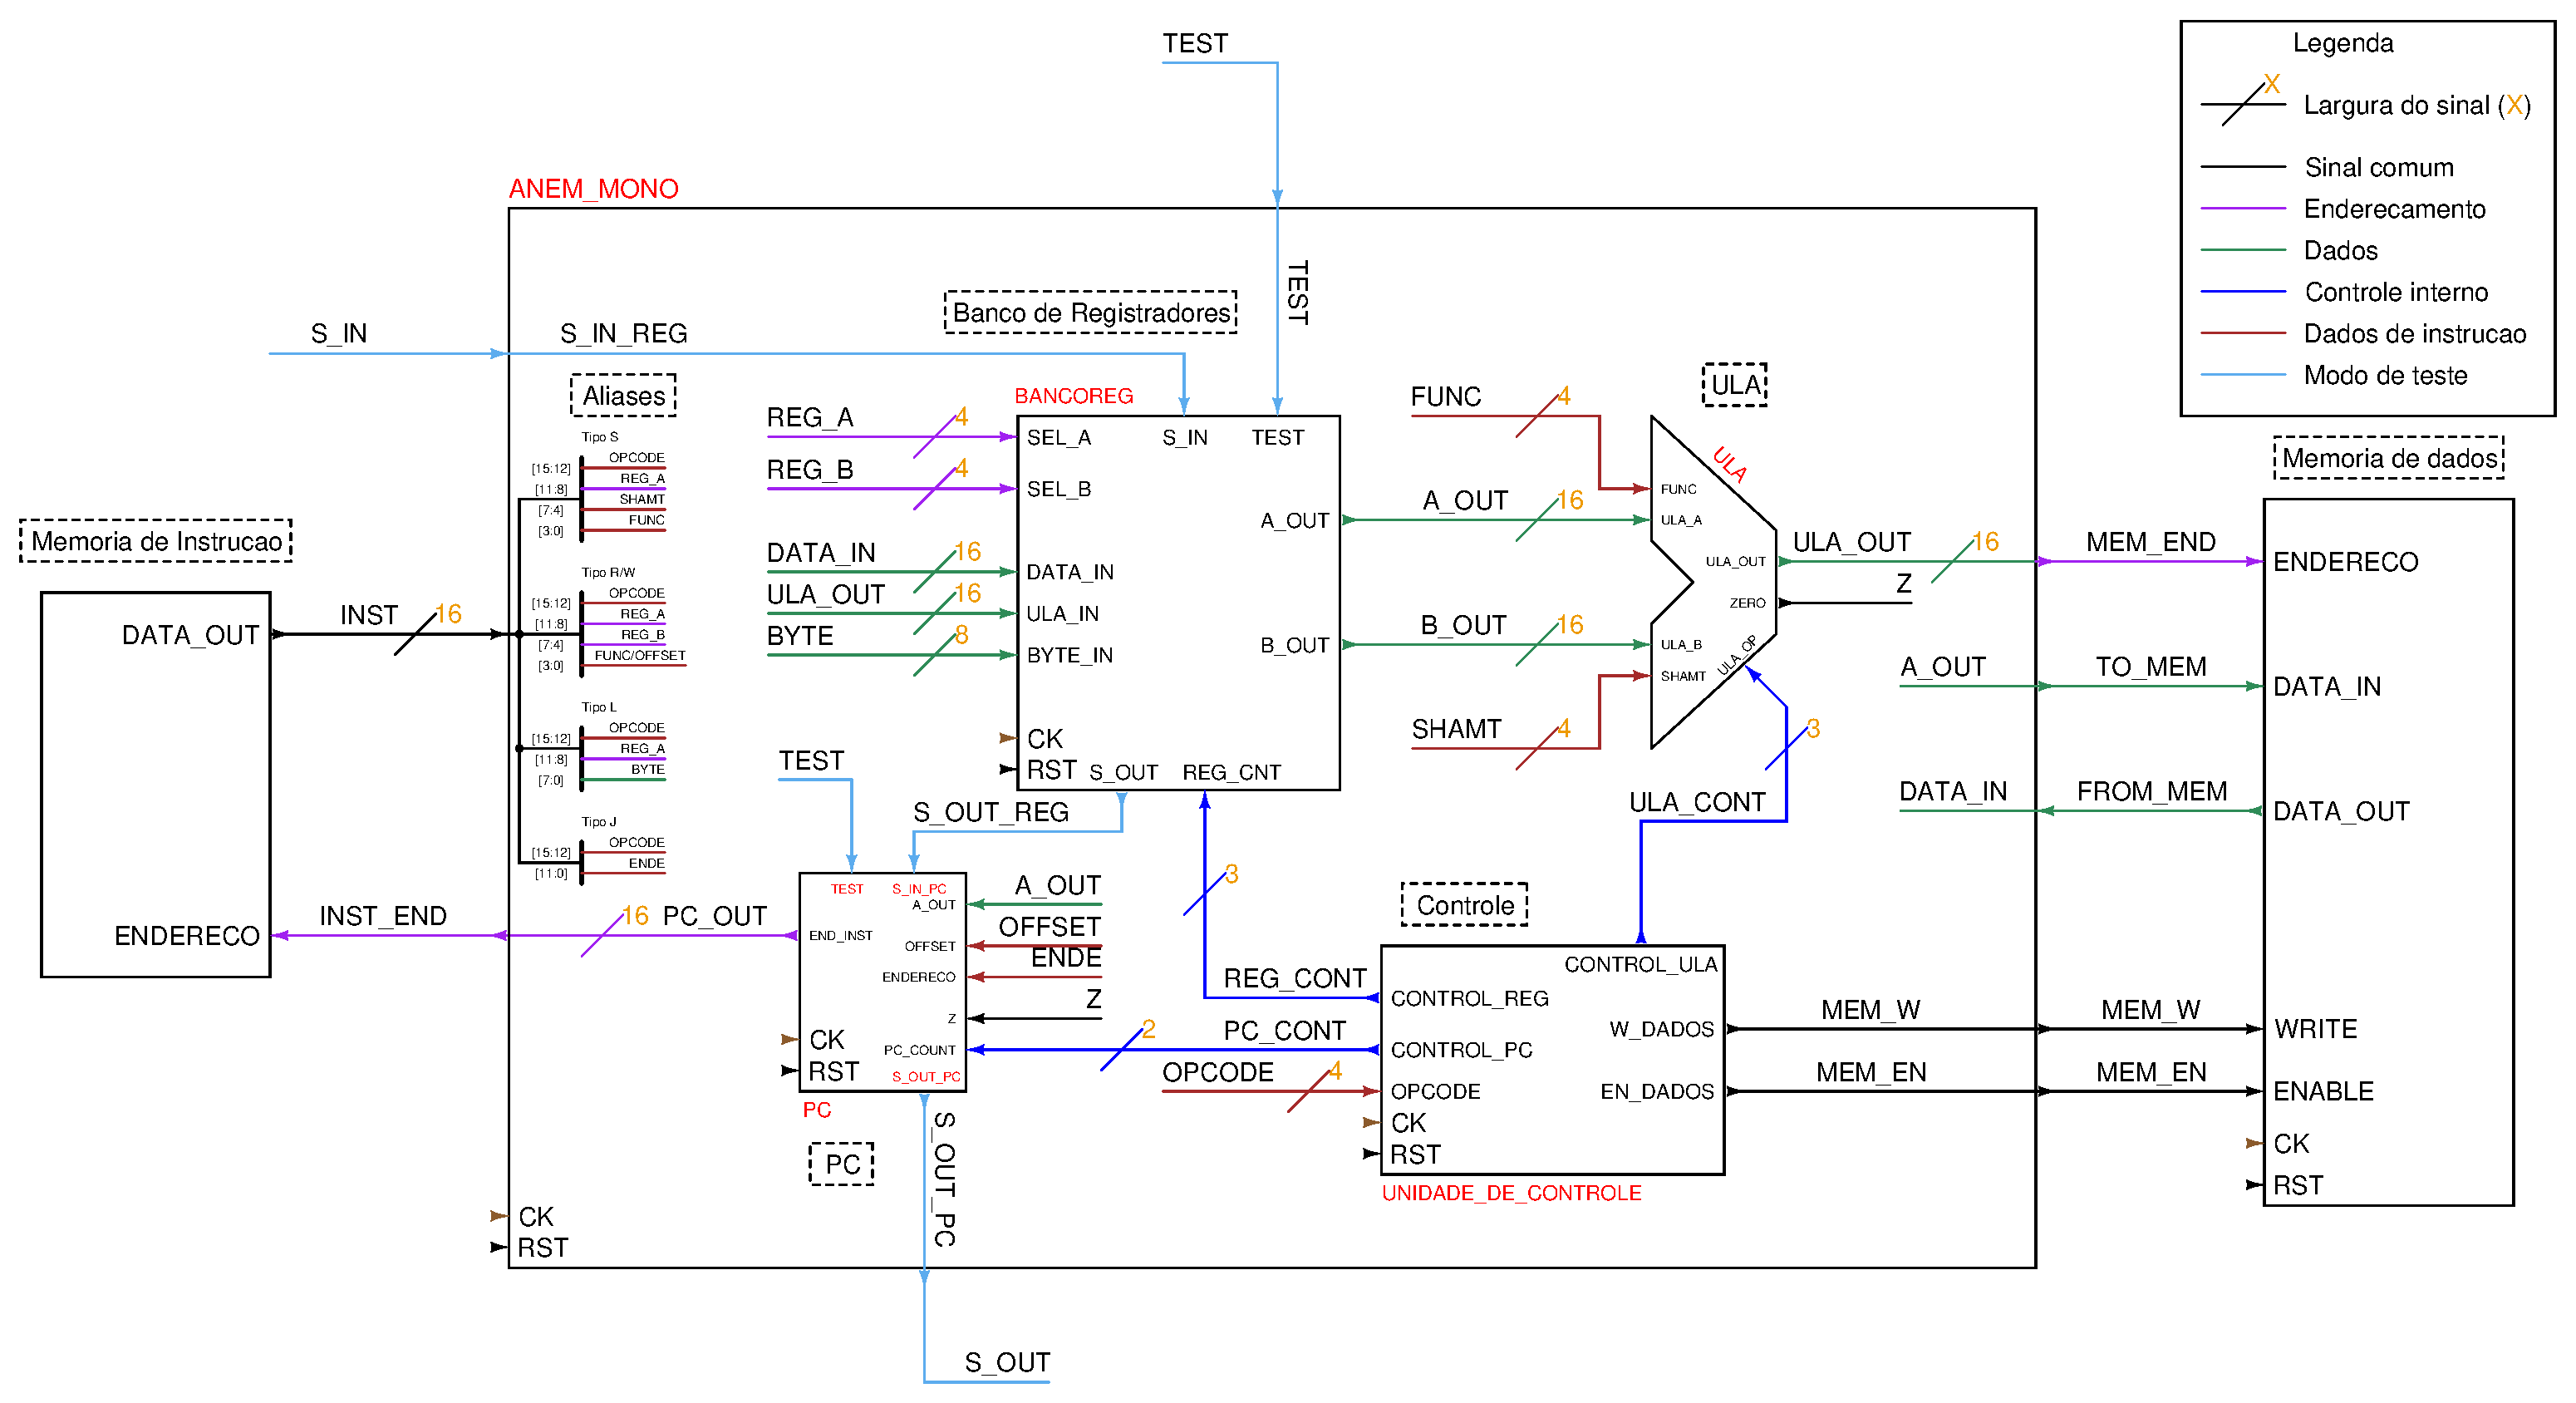
\includegraphics[scale=0.35]{../media/anem_mono_schem.ps}
%\caption{O processador ANEM16 versão mono-ciclo}
%\end{figure}

\subsection{O ANEM-HBUS}

A variação ANEM-HBUS, visa a simplicidade e economia de código, uma vez que os microcontroladores utilizados preferencialmente nos dispositivos HBUS são escolhidos para ter baixo custo e por consequência tem memórias pequenas.

O ANEM-HBUS utiliza palavras de 8-bits. As instruções ainda são de 16-bits. O banco de registradores é composto por 16 registradores de 8 bits e o contador de programa é de 16 bits. O registrador final do banco é fixo no valor zero e é somente para leitura.

Além do banco de registradores, o ANEM-HBUS conta com dois registradores auxiliares, \textbf{HI} e \textbf{LO}.

\subsection{Memória de instrução}

A memória de instrução é um vetor de palavras armazenado em espaço de código, ou seja, é localizado na memória FLASH do microcontrolador. Através de manipulação é possível apagar e re-escrever este conteúdo em tempo de execução. Isto possibilita o \textit{upload} de nova programação com o dispositivo em funcionamento.

O procedimento de \textit{upload} para a execução do microcódigo e re-escreve a memória de instruções. Após isto ser executado com sucesso, o novo microcódigo começa a ser executado. Efetivamente, a \textit{soft-cpu} sofre um RESET.

O upload é conseguido utilizando-se de um \textit{Endpoint} HBUS, conceito já explicado em capítulo anterior. Este endpoint contém a função que realiza a escrita na memória constante de instrução.

\subsection{Instruções disponíveis no microcódigo}

São listadas e discutidas as instruções disponíveis ao usuário. O conjunto de instruções é dividido em tipos, sendo eles:

\begin{itemize}

\item R: Instruções aritméticas
\item S: Instruções de deslocamento
\item J: Instruções de salto incondicional
\item W: Instruções de memória e saltos condicionais
\item L: Instrução para carregamento imediato de valor
\item I: Instrução para geração de interrupções

\end{itemize}

Cada tipo tem um padrão diferente de divisão e utilização dos bits na palavra de instrução. A tabela \ref{tab:inst} detalha as instruções.

\begin{table}[H]
\caption{Instruções disponíveis no microcódigo}
\label{tab:inst}
\begin{tabular}{c c c c}
\hline
Instrução	&	Tipo		&	Descrição\\
\hline
AND			&	R		&	Operação lógica\\
OR			&	R		&	Operação lógica\\
NOT			&	R		&	Operação lógica\\
XOR			&	R		&	Operação lógica\\
ADD			&	R		&	Adição\\
SUB			&	R		&	Subtração\\
MULT			&	R		&	Multiplicação\\
SLT			&	R		&	Compara dois valores\\
DIV			&	R		&	Divisão\\
\hline
SHR			&	S		&	Deslocamento para a direita\\
SHL			&	S		&	Deslocamento para a esquerda\\
ROR			&	S		&	Rotação no sentido da direita\\
ROL			&	S		&	Rotação no sentido da esquerda\\
\hline
J			&	J		&	Salto incondicional\\
JAL			&	J		&	Jump-and-link: salva PC atual nos registradores 13 e 14 e pula\\
\hline
LW			&	W		&	Carrega byte da memória virtual\\
SW			&	W		&	Escreve byte na memória virtual\\
BEQ			&	W		&	Salta em caso de igualdade\\
JR			&	W		&	Salta para endereço contido em registrador\\
\hline
LIW			&	L		&	Carrega valor em registrador imediatamente\\
\hline
INT			&	I		&	Gera interrupção\\
\hline
MFHI			&	M		&	Copia conteúdo do registrador HI\\
MFLO			&	M		&	Copia conteúdo do registrador LO\\
LHL			&	M (M1)	&	Carrega registradores HI e LO\\
LIH			&	M (M1)	&	Carrega registrador HI imediatamente\\
LIL			&	M (M1)	&	Carrega registrador LO imediatamente\\
AIS			&	M (M1)	&	Adiciona valor imediato em HI:LO (com sinal)\\
\end{tabular}
\end{table}

A divisão das palavras de instrução dependendo do tipo de instrução é mostrada a seguir.
%Tabela 1.2 contendo a divisao da palavra de instrucao

\subsubsection{Instruções tipo R}

As instruções tipo R tem estrutura como mostrada a seguir:

\begin{figure}[H]
\centering
\begin{bytefield}[endianness=big,bitwidth=0.035\linewidth]{16}
\bitheader{0-15}\\
\bitbox{4}{OPCODE} & \bitbox{4}{REGA} & \bitbox{4}{REGB} & \bitbox{4}{FUNC}
\end{bytefield}
\caption{Instrução tipo R}
\end{figure}

Estas instruções são operações aritméticas e seus campos são explorados detalhadamente na tabela \ref{tab:ir}. O Opcode das instruções tipo R é 0x0.

\begin{table}[H]
\centering
\caption{Campos da instrução tipo R}
\begin{tabular}{c c p{10cm}}

\hline
Campo	&	Tamanho		&	Função\\
\hline
OPCODE	&	4			&	Informa ao processador o tipo de instrução (R)\\
REGA		&	4			&	Endereço no banco de registradores do operando 1. Também é o destino do resultado\\
REGB		&	4			&	Endereço no banco de registradores do operando 2\\
FUNC		&	4			&	Código que descreve a operação aritmética/lógica a ser realizada\\
\hline
\end{tabular}
\label{tab:ir}
\end{table}

O campo FUNC varia de acordo com a operação a ser realizada. Os valores possíveis e suas correspondentes operações são vistos na tabela \ref{tab:rfunc}.

\begin{table}[h]
\centering
\caption{Instruções tipo R: o campo FUNC}
\begin{tabular}{c l}

\hline
Valor	&	Operação\\
\hline
0x0		&	ADD (adição)\\
0x1		&	SUB (subtração)\\
0x2		&	AND\\
0x3		&	OR\\
0x4		&	XOR\\
0x5		&	NOT\\
0x6		&	MULT (multiplicação)\\
0x7		&	SLT (= 1 se B > A, = 0, c.c.)\\
0x8		&	DIV (divisão)\\
\hline

\end{tabular}
\label{tab:rfunc}
\end{table}

As operações aritméticas tratam os operandos como números sem sinal.

Todas as operações exceto \textbf{DIV} e \textbf{MULT} salvam o resultado da operação no próprio registrador A.

As funções \textbf{DIV} e \textbf{MULT} utilizam os registradores \textbf{HI} e \textbf{LO} da seguinte maneira:

\begin{itemize}

\item \textbf{MULT}: \textbf{HI:LO} = \textbf{REGA} * \textbf{REGB}

\item \textbf{DIV}: \textbf{REGA} = \textbf{HI:LO} \% \textbf{REGB}; \textbf{REGB} = \textbf{HI:LO} / \textbf{REGB};

\end{itemize}

\subsubsection{Instruções tipo S}

As instruções do tipo S são instruções de deslocamento. A estrutura da palavra de instrução é mostrada:

\begin{figure}[H]
\centering
\begin{bytefield}[endianness=big,bitwidth=0.035\linewidth]{16}
\bitheader{0-15}\\
\bitbox{4}{OPCODE} & \bitbox{4}{REG} & \bitbox{4}{SHAMT} & \bitbox{4}{FUNC}
\end{bytefield}
\caption{Instrução tipo S}
\end{figure}

O Opcode destas instruções tem valor 0x1 e seus campos são detalhados a seguir.

\begin{table}[H]
\centering
\caption{Campos da instrução tipo S}
\begin{tabular}{c c p{10cm}}

\hline
Campo	&	Tamanho		&	Função\\
\hline
OPCODE	&	4			&	Informa ao processador o tipo de instrução (S)\\
REG		&	4			&	Endereço no banco de registradores do operando. Também é o destino do resultado\\
SHAMT	&	4			&	Quantidade de deslocamentos realizados\\
FUNC		&	4			&	Código que descreve a operação de deslocamento a ser realizada\\
\hline
\end{tabular}
\label{tab:ir}
\end{table}

\begin{table}[h]
\centering
\caption{Instruções tipo S: o campo FUNC}
\begin{tabular}{c p{6cm}}

\hline
Valor	&	Operação\\
\hline
0x0		&	SHR --- deslocamento a direita\\
0x1		&	SHL --- deslocamento a esquerda\\
0x2		&	ROR --- rotação a direita\\
0x3		&	ROL --- rotação a esquerda\\
\hline

\end{tabular}
\label{tab:sfunc}
\end{table}

As instruções tipo S salvam o resultado das operações no próprio registrador do operando

\subsubsection{Instruções tipo J}

Estas instruções são instruções para a realização de saltos incondicionais. A estrutura da palavra de instrução é mostrada em detalhe:

\begin{figure}[H]
\centering
\begin{bytefield}[endianness=big,bitwidth=0.035\linewidth]{16}
\bitheader{0-15}\\
\bitbox{4}{OPCODE} & \bitbox{12}{ADDRESS}
\end{bytefield}
\caption{Instrução tipo J}
\end{figure}

O campo OPCODE é responsável pela identificação da função da instrução, como já sabido. O campo ADDRESS é o endereço na memória de instrução para qual o processador irá saltar. Em outras palavras esse será o novo valor do \textit{program counter} no próximo ciclo.

As duas instruções utilizadas são descritas:

\begin{table}[H]
\caption{Descrição das instruções tipo J}
\begin{tabular}{c c p{10cm}}
\hline
Instrução 	& 	OPCODE 		&	Descrição\\
\hline
J			&	0x8			&	Salta imediatamente para o endereço dado\\
JAL			&	0x9			&	Jump-and-Link: grava nos registradores 13 e 14 o valor do \textit{program counter} e salta imediatamente para o endereço dado\\
\hline
\end{tabular}
\label{tab:jinst}
\end{table}	 

\subsubsection{Instruções tipo W}

As instruções do tipo W são instruções de salto condicional ou de acesso a memória de programa.

\begin{figure}[H]
\centering
\begin{bytefield}[endianness=big,bitwidth=0.035\linewidth]{16}
\bitheader{0-15}\\
\bitbox{4}{OPCODE} & \bitbox{4}{REGS} & \bitbox{4}{REGD} & \bitbox{4}{OFFSET}
\end{bytefield}
\caption{Instrução tipo W}
\end{figure}

Uma análise dos campos da instrução segue:

\begin{table}[H]
\centering
\caption{Campos da instrução tipo W}
\begin{tabular}{c c p{10cm}}

\hline
Campo	&	Tamanho		&	Função\\
\hline
OPCODE	&	4			&	Informa ao processador o tipo de instrução (S)\\
REGS		&	4			&	Endereço no banco de registradores do registrador fonte\\
REGD		&	4			&	Endereço no banco de registradores do registrador destino\\
OFFSET	&	4			&	Offset para salto ou para ser somado ao endereço de leitura na memória\\
\hline
\end{tabular}
\label{tab:iw}
\end{table}

A terminologia de registrador fonte e registrador destino foi criada para iluminar a operação das instruções.

O registrador \textbf{fonte} é aquele de onde é retirada a informação para a operação de salto ou acesso a memória. No caso das instruções LW e SW, o valor contido no registrador indicado pelo campo da instrução será o endereço da memória a ser lido ou escrito. O registrador destino, no caso da operação de leitura (LW) identifica o registrador no qual será escrito o byte lido da memória. Já para a instrução de escrita (SW), o registrador destino é o registrador que contém o valor a ser escrito na memória virtual. O valor do campo OFFSET é somado ao conteúdo dos registradores que contém os endereços de memória.

Para a operação JR, o registrador de destino perde o sentido e é ignorado, importando apenas o campo de registrador fonte, que deve conter o endereço para onde se deseja saltar. Note que devido a uma limitação das palavras no banco de registrador do ANEM-HBUS, só é possível saltar até a posição 255 da memória de instrução. Esta limitação é relevada, uma vez que o microcódigo não pretende realizar tarefas altamente complexas e por uma questão de limitação em espaço disponível na memória FLASH dos microcontroladores escolhidos, a memória de instrução só é alocada até o tamanho máximo de 256 instruções. O campo OFFSET é somado ao valor do registrador com o endereço da instrução alvo do salto.

Na operação tipo BEQ, os valores contidos nos registradores fonte e destino são comparados, e quando iguais, ocorre o salto para a posição atual do PC mais OFFSET instruções. Mais uma vez, percebe-se uma limitação, já que tendo apenas 4 bits disponíveis, o BEQ é capaz de saltar até apenas 15 instruções a frente da atual. Recomenda-se o uso combinado de uma instrução BEQ que salta para uma instrução tipo J no caso de ser necessário um salto para uma posição mais distante.

\begin{table}[H]
\caption{Descrição das instruções tipo W}
\begin{tabular}{c c p{10cm}}
\hline
Instrução 	& 	OPCODE 		&	Descrição\\
\hline
LW			&	0x5			&	Carrega dados da memória virtual\\
SW			&	0x4			&	Salva dados na memória virtual\\
JR			&	0x7			&	Salta para posição indicada por registrador\\
BEQ			&	0x6			&	Salto condicional dependendo do valor dos registradores\\

\hline
\end{tabular}
\label{tab:winst}
\end{table}	 

\subsubsection{Instrução tipo L}

A instrução do tipo L é a instrução LIW. Os seus campos são mostrados:

\begin{figure}[H]
\centering
\begin{bytefield}[endianness=big,bitwidth=0.035\linewidth]{16}
\bitheader{0-15}\\
\bitbox{4}{OPCODE} & \bitbox{4}{REG} & \bitbox{8}{DATA}
\end{bytefield}
\caption{Instrução tipo L}
\end{figure}

Esta instrução realiza o carregamento imediato de um byte, contido no campo DATA no registrador indicado pelo endereço no campo REG.

\subsubsection{Instrução tipo I}

A instrução do tipo I é a instrução INT. Esta instrução deflagra uma interrupção do barramento HBUS.

\subsubsection{Instruções tipo M}

As instruções do tipo M são destinadas a movimentação e manipulação de dados dos registradores \textbf{HI} e \textbf{LO}. Este tipo de instrução tem alguns subtipos:

\begin{figure}[H]
\centering
\begin{bytefield}[endianness=big,bitwidth=0.035\linewidth]{16}
\bitheader{0-15}\\
\bitbox{4}{OPCODE} & \bitbox{8}{---} & \bitbox{4}{REG}
\end{bytefield}
\caption{Instrução tipo M}
\end{figure}

\begin{figure}[H]
\centering
\begin{bytefield}[endianness=big,bitwidth=0.035\linewidth]{16}
\bitheader{0-15}\\
\bitbox{4}{OPCODE} & \bitbox{4}{MOP} & \bitbox{8}{DATA}
\end{bytefield}
\caption{Instrução subtipo M1}
\end{figure}

\begin{table}[H]
\caption{Descrição das instruções tipo M}
\begin{tabular}{c c p{10cm}}
\hline
Instrução 	& 	OPCODE 		&	Descrição\\
\hline
MFHI			&	0xA			&	Copia conteúdo do registrador HI para REG\\
MFLO			&	0xB			&	Copia conteúdo do registrador LO para REG\\
Subtipo M1	&	0xD			&	Ver tabela abaixo\\

\hline
\end{tabular}
\label{tab:winst}
\end{table}	 

\begin{table}[H]
\caption{Descrição das instruções subtipo M1}
\begin{tabular}{c c p{10cm}}
\hline
Operação 	& 	MOP 		&	Descrição\\
\hline
LHL			&	0x0			&	Carrega registradores HI e LO de DATA[7..4],DATA[3..0]\\
LIH			&	0x1			&	Carrega registrador HI imediatamente com DATA\\
LIL			&	0x2			&	Carrega registrador LO imediatamente com DATA\\
AIS			&	0x3			&	Adiciona valor imediatamente em HI:LO (com sinal)\\

\hline
\end{tabular}
\label{tab:winst}
\end{table}	 

\subsection{A memória virtual}
A memória de dados é mapeada virtualmente a partir dos objetos HBUS declarados pelo dispositivo. Isto dá acesso de leitura e escrita aos objetos. O usuário não tem acesso a memória RAM do microcontrolador, sendo obrigado a limitar-se ao banco de registradores para realizar suas tarefas.

Com o intuito de simplificar a implementação e não impor grandes dificuldades ao processador hóspede (microcontrolador), é assumido que cada objeto HBUS tem um tamanho de 4 bytes.

É uma limitação da especificação HBUS que o objeto tenha no máximo 4 bytes, então não haverá problemas de objetos maiores que os 4 bytes para endereçamento. No caso de o objeto possuir menos de 4 bytes, as tentativas de operações fora deste espaço são simplesmente ignoradas.

Observe que o usuário tem apenas 8 bits para endereçar os objetos, o que dá um total de $\frac{2^8}{4} = 64$ objetos no máximo. Não é esperado que o dispositivo possua essa quantidade de objetos, devido a natureza da especificação HBUS.

\subsection{A operação da máquina virtual}

Um outro termo muito usado para o processador emulado em software é \textit{máquina virtual}.

A máquina virtual que emula o ANEM-HBUS é implementada nos arquivos \textit{microcode.h} e \textit{microcode.c}. 

As funções e estruturas de dados que controlam a operação e o fluxo de dados são descritos brevemente a seguir.

A estrutura de execução é basicamente dividida em duas funções, sendo uma de inicialização e outra que executa um ciclo da máquina virtual.

\subsubsection{Máquina virtual: registradores, estruturas de dados e funções}

Os registradores de dados e também de status do processador são implementados através da estrutura que é mostrada a seguir:

\begin{minted}[linenos]{c}

typedef struct CPUEMU_S
{
	//registradores
	word PC;			//program counter
	
	byte BANK[16];	//banco de registradores
	byte ALUREG; 	//emula a saida da ULA
	
	byte STATUS;		//registrador de status
	
	UCODE_INSTRUCTION INST; //registrador de instrução
	
} UCODE_CPUDATA;

\end{minted}

O processo de inicialização é realizado pela função UCODE\_STARTUP() e os ciclos são gerados pela função UCODE\_CYCLE().

\subsubsection{A função UCODE\_STARTUP()}

Esta função é chamada na inicialização do código do processador hospedeiro. Ela é responsável pela inicialização de todos os registradores da máquina virtual.

Esta função também é chamada no caso de o microcódigo ser atualizado de forma on-line. A máquina virtual é então re-inicializada.

\subsubsection{A função UCODE\_CYCLE()}

Esta função simula os ciclos do processador ANEM-HBUS. Dentro dela são simuladas as etapas de FETCH, DECODE e as operações resultantes,dependendo da instrução que for interpretada no ciclo.

A etapa de FETCH é simulada copiando-se uma palavra de instrução da memória de instrução implementada, em acordo com o valor atual do registrador PC.

A etapa de decode é simulada facilmente e as operações instruídas são realizadas em seguida. Estas operações são realizadas utilizando-se de operadores básicos da linguagem C, no caso de instruções que não envolvam acesso à memória virtual.

No caso de acesso à memória virtual, outras funções, que simulam o acesso de leitura e escrita, são chamadas. Estas funções serão discutidas a seguir.

\subsubsection{A função UCODE\_PAUSE\_()}

Esta função seta um flag no registrador de status que faz com que a operação da máquina virtual cesse. Isto é muito útil no caso de o processador hospedeiro necessitar parar a operação por algum motivo qualquer e é também necessário no caso de ocorrer um update on-line do microcódigo, onde a máquina virtual deve parar para que a memória de instrução possa ser re-escrita.

\subsubsection{A função UCODE\_UNPAUSE()}

Esta função é complementar à anterior, restaurando a operação da máquina virtual.

\subsubsection{As funções UCODE\_LOAD\_DATA() e UCODE\_SAVE\_DATA()}

Estas funções simulam o acesso a memória de programa do ANEM-HBUS, que é a memória virtual onde estão mapeados os dados dos objetos, organizada no esquema já explicado.

Dentro destas funções são chamados os métodos de leitura e escrita especificados pelo próprio objeto, de maneira que a leitura e escrita realizadas pela máquina virtual não diferem de uma leitura/escrita realizada através do barramento HBUS.

\section{O acesso à memória de instrução}

A memória de instrução é por definição alocada em uma parte reservada na FLASH do microcontrolador.
É possível a escrita nesta porção da memória mesmo em tempo de execução.

O acesso neste caso é de escrita e é realizado através de um \textit{endpoint} registrado no dicionário de \textit{endpoints} do dispositivo. Os dados para a memória de instruções são enviados em blocos de 64 bytes conforme a necessidade.

A operação pode ser realizada sem a necessidade de reinicialização do dispositivo, possibilitando a atualização sob demanda do microcódigo, com efeito imediato, através dos procedimentos descritos neste capítulo.
